\section{What do you do with multicore?}

\begin{frame}[t]{Impact of multicores}
\begin{itemize}
\item Increase \textgood{throughput}:
  \begin{itemize}
    \item More transactions per second.
    \item Mostly \textmark{concurrent programming}.
  \end{itemize}

\item Increase performance
  \begin{itemize}
    \item Faster execution of a task.
    \item Mostly \textmark{parallel programming}.
  \end{itemize}
\end{itemize}
\end{frame}

\begin{frame}[t]{C++11/14}
\begin{itemize}
  \item Focused in providing the concurrency building blocks.
  \item Main features:
    \begin{itemize}
      \item Clear definition of the memory model.
      \item Support for TLS (\cppkey{thread\_local}).
      \item Concurrency portable abstractions:
        \begin{itemize}
          \item \cppid{std::thread}.
          \item \cppid{std::mutex}, \cppid{std::timed\_mutex}, \ldots
          \item \cppid{std::condition\_variable}, \cppid{condition\_variable\_any}.
          \item \cppid{std::unique\_lock}, \ldots
          \item \cppid{std::promise}, \cppid{std::future}, \cppid{std::packaged\_task}.
        \end{itemize}
      \item Low level portable \emph{lock-free} abstractions:
        \begin{itemize}
          \item \cppid{std::atomic}.
          \item \cppid{std::memory\_order}.
        \end{itemize}
    \end{itemize}
\end{itemize}
\end{frame}

\begin{frame}[t]{Where do I get this?}
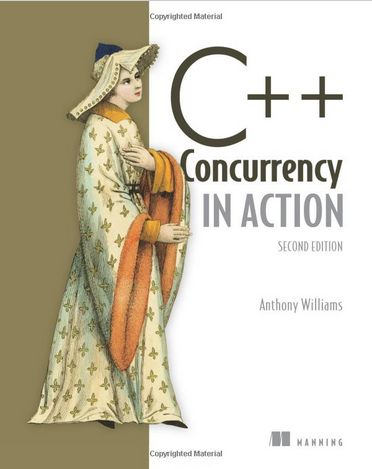
\includegraphics[height=.9\textwidth]{images/williams-book.png}
\end{frame}
